
\section{Trénovacia databáza zbraní}
\label{sec:databaza}
Pre správne trénovanie klasifikátorov a neurónových sieti je dôležité mať dáta v dostatočnom počte a správne označené.
Trénovacia databáza je získana z niekoľkých zdrojov.
\begin{enumerate}
    \item[$\bullet$] \textbf{IMFDB}\footnote{\url{http://www.imfdb.org/wiki/Main_Page}} - je databáza záberov z filmov v ktorých sa nachádzajú zbrane.
    Obsahuje nie len celkové scény ale aj samostatné obrázky zbraní ktoré sa v danej scéne nachádzajú.
    Pre túto prácu je potrebné aby daný obrázok obsahoval iba zbraň, preto je potrebné obrázky z tejto databázy ručne odfiltrovať na samotné zbrane a scény so zbranami.
    Následne ich potom zaradiť do správnej kategórie na krátke a dlhé.
    \item[$\bullet$] \textbf{ImageNet}\footnote{\url{http://www.image-net.org/}} - je databáza obrázkov ktorá obsahuje viac ako 14 miliónov obrázkov vo viac ako 21000 kategóriach.
    Výhodou tejto databázy je že obrázku už patria do určenej kategórie a tak nieje potrebné ich ručné prechádzať a kategorizovať.
    \item[$\bullet$] \textbf{Google}\footnote{\url{http://www.google.com}} - pre doplnanie a zväčšenie počtu obrázkou je môžné použiť google vyhľadávanie.
    Tak ako v prípade IMFDB bude potrebné obrázky ručne kategorizovať.
    \item[$\bullet$] \textbf{Free3D}\footnote{\url{https://free3d.com/3d-models/weapons}} - databáza voľne dostupných 3D modelov zbraní s textúrami v rôzných formátoch.
\end{enumerate}

Databáza zbraní z prvých 3 zdrojov je možné použit na klasficikáciu zbraní do 2 kategórií na krátke a dlhé zbrane.
Pre trénovanie neurónových sieti na určenie náklonu zbrane v obraze bude potrebné použiť 3D modely zbraní a následne z nich vygenerovať
    obrázky zbraní v požadovaných natočeniach zbrane v obraze.

\subsection{Generovanie dát z 3D modelov}
\label{subsec:generovanie3d}
Generovanie obrázkov pre určenie náklonu zbrane v scéne bude prebiehať pomocou databázy 3D modelov zo zdroja Free3D.
Následne sa použije software od Ing. Tomáša Goldmanna do ktorého je potrebné vložiť 3D model vo formáte g3db a pozadie scény.

Kedže 3D modely ktoré budú použité niesu v požadovanom formáte, je potrebné ich prekonvertovať, to je môžné urobiť
    pomocou nástroja \textbf{fbx-conv}\footnote{\url{https://github.com/libgdx/fbx-conv}}.
Tento nástroj podporuje konvertovanie 3D modelov z formátu fbx alebo obj do požadovaného formátu g3db.

\subsection{Augmentácia obrázkov}
\label{subsec:augmentacia}
Ako bolo opísane v kapitole \ref{sec:preprocessing} jedna z možností zväčšenia počtu vstupných dát a zlepšenia generalizácie pri klasifikácií je augmentácia vstupných dát.
V tejto práci môžeme rozdeliť augmentáciu dát do dvoch skupín, prvý druh augmentácie bude prebiehať pre trénovanie klasifikátorov ktoré
    určuju typ zbrane, druhý druh augmentácie bude prebiehať pri obrázkoch určených pre náklon zbrane.

Pri augmentácií dát pre klasifikovanie dvoch tried, na krátke a dlhé zbrane, prebehne niekoľko transfomácií obrázka.
\begin{enumerate}
    %\item[$\bullet$] \textbf{priblíženie} - priblíženie alebo oddialenie vstupného obrázku
    \item[$\bullet$] \textbf{Rotácia} - obrázky budú rotované o náhodny uhol v rozmedzí 0-180 stupňov.
    \item[$\bullet$] \textbf{Preklopenie} - vertikálne alebo horizonálne preklopenie obrázka.
    \item[$\bullet$] \textbf{Posun} - posun obrázka po x-ovej a y-ovej osi.
    \item[$\bullet$] \textbf{Výplň} - pri rotácií alebo posunu obrázku môže vzniknúť čierna plocha pixelov, tieto čierne pixely je potrbné vyplniť.
    Tieto čierne pixely budú doplnené hraničným pixelom obrázka ktorý bude nakopírovaný až po nový okraj.
\end{enumerate}

\begin{figure}[H]
    \centering
    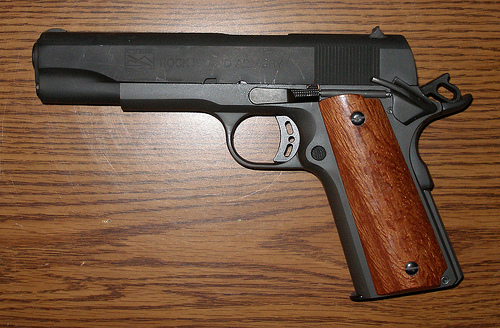
\includegraphics[width=0.4\textwidth]{weapons/weapon}
    \qquad
    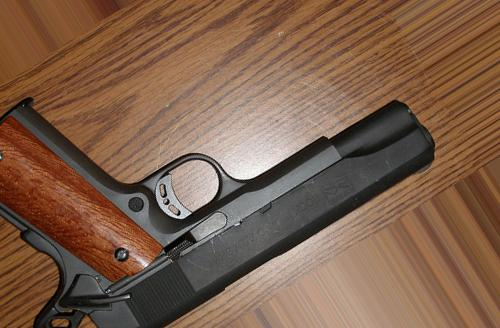
\includegraphics[width=0.4\textwidth]{weapons/weapon-augmented}
    \caption{Pôvodny obrázok (vľavo), augmentovaný obrázok (vpravo)}
    \label{pic:imageAugmented}
\end{figure}

Druhý typ augmentácie dát prebieha pri obrázkoch ktoré boli vygenerované pomocou 3D modelu.
Kedže nieje potrebné generovať všetky polohy otočenia od 0 po 360 stupňov, stačí vygenerovať dáta v polohách od 0 po 90 stupňov a od 270 do 359 stupňov
    zvyšné polohy je možné dogenerovať pomocou transformácie obrázka, pomocou vertikálneho alebo horizonálneho preklopenia.
Avšak v tomto prípade je potrebné po transformácií obrázka vyrátať novú hodnotu uhla transformovaného obrázka, to je môžené dosiahnuť pomocou niekoľkých
    jednoduchých vzorcov.

\textbf{Roll}, pri natočení modelu v ose roll, je potrebné aplikovať horizontálne preklopenie obrázka.
Následne uhol transformovaného obrázka $trans\_angle$ bude vypočítaný z pôvodneho uhla $angle$ podľa:
\begin{equation}
    trans\_angle = -angle + 540 \quad ak \; 270 \leq angle \leq 359
\end{equation}
\begin{equation}
    trans\_angle = abs(angle - 180) \quad ak \; 0 \leq angle \leq 90
\end{equation}

\begin{figure}[H]
    \centering
    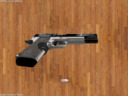
\includegraphics[width=0.3\textwidth]{weapons/roll_300}
    \quad
    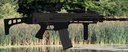
\includegraphics[width=0.3\textwidth]{weapons/roll_0}
    \quad
    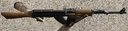
\includegraphics[width=0.3\textwidth]{weapons/roll_70}
    \caption{Natočenie zbrane v ose roll, 300 stupňov(vľavo), 0 stupňov(v strede), 70 stupňov(vpravo)}
    \label{pic:rollrotation}
\end{figure}

\textbf{Yaw}, pri natočení v ose yaw, sa aplikuje vertikálne preklopenia obrázka.
Uhol transformovaného obrázka sa vypočít podľa:
\begin{equation}
    trans\_angle = abs(angle - 540) \quad ak \; 270 \leq angle \leq 359
\end{equation}
\begin{equation}
    trans\_angle = abs(angle - 180) \quad ak \; 0 \leq angle \leq 90
\end{equation}

\begin{figure}[H]
    \centering
    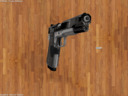
\includegraphics[width=0.3\textwidth]{weapons/yaw_300}
    \quad
    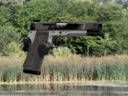
\includegraphics[width=0.3\textwidth]{weapons/yaw_0}
    \quad
    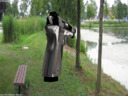
\includegraphics[width=0.3\textwidth]{weapons/yaw_75}
    \caption{Natočenie zbrane v ose yaw, 300 stupňov(vľavo), 0 stupňov(v strede), 75 stupňov(vpravo)}
    \label{pic:yawrotation}
\end{figure}

\textbf{Pitch}, v ose pitch postačuje vygenerovať obrázok zbrane s náklonom 0 stupňov so smerovaním hlavne zbrane doprava.
Počas augmentácie dát sa môže aplikovať horizontálne preklopenie a následne sa tento vstupný obrázok otočí o náhodny uhol.
Preto nieje potrebný žiaden další prepočet uhla.

\begin{figure}[H]
    \centering
    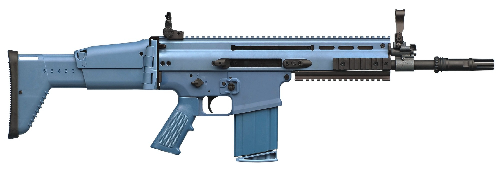
\includegraphics[width=0.3\textwidth]{weapons/pitch_0}
    \quad
    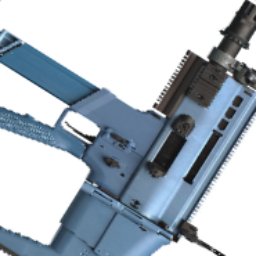
\includegraphics[width=0.2\textwidth]{weapons/pitch_60}
    \quad
    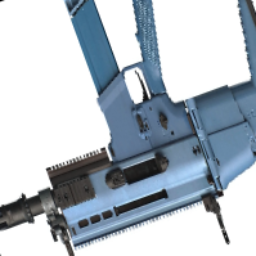
\includegraphics[width=0.2\textwidth]{weapons/pitch_200}
    \caption{Natočenie zbrane v ose pitch, 0 stupňov(vľavo), 60 stupňov(v strede), 200 stupňov(vpravo)}
    \label{pic:yawrotation}
\end{figure}
